\chapter{Research Context}
\graphicspath{{Chapter2/Figs/}{Chapter2/Figs/}}

This chapter describes the research question's context and the current literature findings. The reader is educated on neuroscientific limitations, the state of current non-invasive and unidirectional BCIs, the paradigm shift in developing cloud-based and production-ready software and the implications of a N/CI for web applications that go hand in hand with BCI technologies.

\section{Limitations of BCIs}
\label{chapter2-limitations-of-bcis}

The possibilities of BCIs are not without limitations. In addition to the hardware limitations, the author attempts to address a broader issue related to neuropsychology that directly correlates with the software aspects, in addition to the challenges of computability.

\subsection{Decoding brain data}
\label{chapter2-decoding-brain-data}

As outlined in the previous chapter, a holistic view of BCI must take into account the aspect of decoding measured neural data and making it intelligible to computer software. It is important to emphasise that the task of decoding neural data is different from decoding thoughts, which is a critical factor for software. Moreover, decoding neural data and extracting the thoughts behind it so that the software can understand them are disciplines on their own. For example, getting computers to recognise letters written on a photograph is a very different problem from reading the written words in the sentences (i.e. computer vision and natural language processing).

Another part is understanding the sentences and their meaning, as in natural language understanding (NLU). NLU is considered an AI-hard problem, which means that the difficulty of these computational problems is equivalent to solving the central problem of artificial general intelligence\footnote{Based on the assumption that general human-level intelligence is computable.} (AGI) \citep{demasi_theoretical_2010}. Understanding less structured data, such as EEG data, is more complicated than understanding structured and human-generated syntax such as written language because it contains more hidden features than a paragraph of text. As a result, the author assumes that understanding brain data might be considered an AI-hard problem.

\subsection{Abstract thoughts}
\label{chapter2-abstract-thoughts}

\begin{figure}[ht]
  \centering
  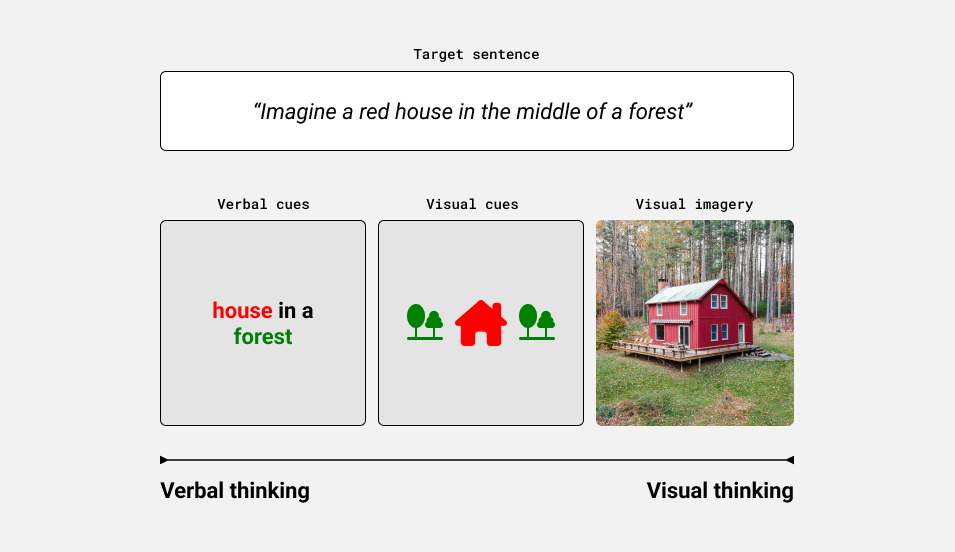
\includegraphics[width=\linewidth]{visual-thinking.png}
  \caption{Difference between verbal and visual thinking using the target sentence of a red house in the middle of a forest (own representation, 2022).}
  \label{fig:visual-thinking}
\end{figure}

To further emphasise the complexity of interpreting neural data, a practical example will be presented: Imagine a red house in the middle of a forest. Depending on the individual thought process, one might imagine the house with temporary visual imagery in mind, as in visual thinking, or one might imagine it more verbally, such as conceptually comprehending each word sequentially of what a red house is and that it is located in a forest \citep{amit_asymmetrical_2017}. Additionally, it should also be addressed that different types of thoughts exist at different levels of abstraction and complexity. One can assume that the visual image of a red house in the forest is more abstract and far-fetched than, say, the movement of one's own thumbs, which has a clear physical counterpart. It gets even more complicated when one imagines concepts that are inconceivable to visualise, such as the idea of a company. A company is only an abstract, collectively agreed upon concept without a physical counterpart\footnote{Some people might think of a company building when imaging a company, others might imagine their website, their logo or physical products etc.} and is, therefore, even less straightforward and more complex to decode the meaning of measured brain activity than the other mentioned examples of the red house.

\subsection{Technological limitations}
\label{chapter2-technological-limitations}

\begin{figure}[ht]
  \centering
  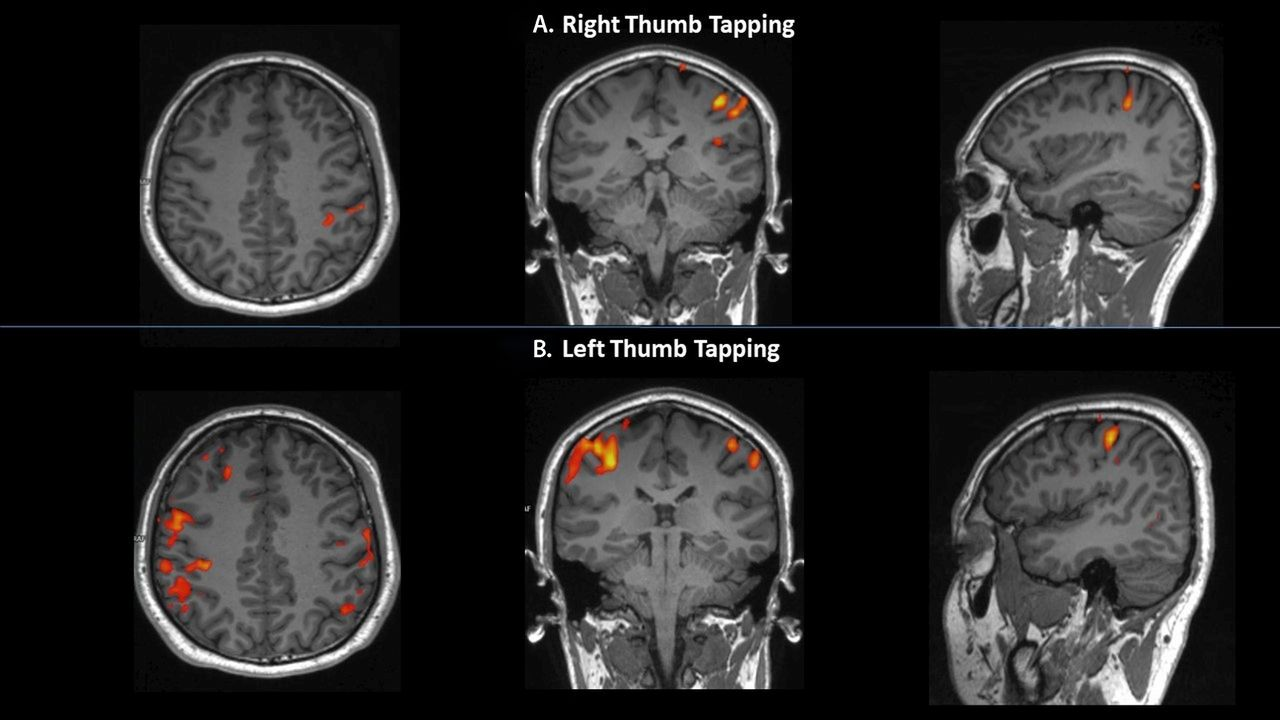
\includegraphics[width=\linewidth]{fmri-scan.jpg}
  \caption{Image of localised activation of neurons during right and left thumb movement using functional magnetic resonance imaging (fMRI) \citep{rashid_bilateral_2018}.}
  \label{fig:fmri-scan}
\end{figure}

Most functional tasks of the brain are localised, which means that these signals are generated by local brain areas that can be identified, such as the motor cortex, which has been shown to be responsible for muscle movement as shown in \autoref{fig:fmri-scan} \citep{rashid_bilateral_2018}. Examining the areas of the brain responsible for activating individual muscle strands can yield a comparable response of muscle stimulation in the brain and thus be measured as output for software to move a prosthesis, for example. However, the more specific, less functional, more behavioural and abstract the thoughts are, the less the brain areas are spatially visible. The intent of identifying, for example, the thought of a red house in a forest in verbal thought, the author identified three technological problem statements:

\begin{itemize}
  \item To understand single thoughts, it is essential to have sufficiently clear data from experiments with a certain level of detail (e.g., at the level of detail related to the firing of action potential of individual neurons) as well as temporal precision (an action potential takes about 1 ms to arise) to perform studies to extract possible localisation of individual thoughts. Current neuroimaging technologies cannot capture every process in sufficient detail of the entire brain at once to extract the activity of, e.g. individual neurons while also having high temporal precision.
  \item Even if we could measure every single neuron in the brain with high temporal precision, we would have an extreme amount of data generated concisely. Let us say we would collect a float per neuron that represents the rate of change in voltage with respect to time with a frequency of 1 ms and then record each neuron in the brain a million times a second, taking into account that the average human brain has around 86 billion neurons; we would generate 305.53337637684 petabytes of data per second. This is currently not feasible for commercially available storage and processing resources.
  \item Even if we have the technology, it is a challenge because reproducibility of experiments is very difficult for neuroscientific studies. It is probably impossible to generate clean-slate neural data that is comparable to previously recorded data. Our neurophysiological brain structure changes over time due to neuroplasticity \citep{puderbaugh_neuroplasticity_2022}, and we are in different states of mind every millisecond of our existence, which can have different influences, such as insufficient sleep, something disturbing someone, mental distraction due to an important event that may have occurred since the last measurement, or a salient thought that occurs during a measurement.
\end{itemize}

\subsection{Lack of data}
\label{chapter2-lack-of-data}

As pointed out in the previous section, points 2 and 3 depend on advances in data storage systems or the possibility that we do not actually need such precise brain data to understand single thoughts. However, to address point 1, some promising solutions already exist for measuring large parts of the brain with high temporal and spatial precision, such as time-domain functional near-infrared spectroscopy (TD-fNIRS), which Kernel employs in its Kernel Flow device \citep{ban_kernel_2021}. The TD-fNIRS system detects changes concentrations of oxygenated (oxyHb) and deoxygenated brain cell activity by using near-infrared light in response to neuronal activity. This is a newer and more promising technology for measuring the full spectrum of neuroimaging of brain activity when compared to e.g. EEG. According to Kernel's, the precision of TD-fNIRS is sufficient for better understanding the brain and using it for BCI applications. They, however, claim that collecting and organising longitudinal brain data from a variety of subjects is the key to solving the most difficult challenges in neuroscience \citep{kernel_hello-humanitypdf_nodate}.

Based on Kernel's claim, a recent publication from 2022 also claims that even data sets with several hundred people are too tiny to consistently offer insights about the brain \citep{marek_reproducible_2022}. As a result, most published neuroscience studies with dozens or even hundreds of people could all be incorrect. In such research, variations in brain structure and activity have been linked to variances in cognitive capacity, mental health, and other behavioural features. Numerous studies, for example, have revealed brain structure or activity patterns that may help distinguish persons with depression from those who are not. Neuromarkers of behavioural features is frequently sought in studies. The recent publication from \citeauthor{marek_reproducible_2022} claims that most of these so-called neuro markers would not work when the collected data set is more extensive, which prose a general problem for the field of neuroscience.

This is both fascinating and a significant constraint for BCIs, because understanding the brain is essential to making sense of the measured and classified data for interfacing with it. Therefore a large amount of brain data collected in reproducible experiments is a must for production-ready and mainstream-ready BCIs. UK Biobank's collection of brain scans is one of the first efforts to solve this problem \citep{noauthor_imaging_nodate}, but it is still far from what we might need. Marek himself claims that we might even need millions of data sets to start understanding the brain \citep{callaway_can_2022}. This is where customer-oriented BCIs could come into play, because the adoption rate of a device capable to be used in everyday life is higher than that of experimental subjects, making it more likely to generate larger and longitudinal data sets. We will further discuss this in a later chapter.

\section{BCI landscape}
\label{chapter2-research-landscape}

In this section we will discuss the current state of real-life and non-invasive BCIs, their applications and the distinctions that lie within their software offerings.

\subsection{Real-world BCI applications}
\label{chapter2-real-world-bci-applications}

As mentioned in \autoref{chapter1-background}, consumer-oriented BCI products are already commercially available. Based on Google Trends\footnote{Google Trends: https://trends.google.com} the products from OpenBCI are most likely the most popular. OpenBCI does not provide a specific use case, but rather a hardware and software stack that is universally applicable. It can be used in research where EEG is to be used or in the development of BCI applications. Several research or neurofeedback apps have been created using OpenBCI's products \citep{openbci_openbci_nodate}. Taking this information into consideration, we can see that the OpenBCI customer is responsible for developing their own BCI application or incorporating it into their research, rather than having a sophisticated and end-user application from OpenBCI.

Another example is NextMind, which was recently acquired by Snapchat \citep{heater_snap_2022}. They do not have an end-user application for their BCI\footnote{NextMind and OpenBCI have both a graphical user interface (GUI) application for the control and quality check of their hardware, but neither is intended for end-users.}, but they do offer an SDK for the Unity real-time engine to use their technology for brain-controlled actions in video games. One significant difference between NextMind and OpenBCI is that NextMind includes built-in classification of brain waves captured by hardware, in this case classification of active visual focus on virtual objects based on steady state visual evoked potentials (SSVEP). Because their business model was presumably based on the unique selling point of their active visual focus classifier, NextMind did not provide access to the raw EEG data collected by the sensors. Nonetheless, NextMind's product is less focused on a specific use case, as its applicability is limited to game developers.

\begin{figure}[!htb]
  \minipage{0.32\textwidth}
  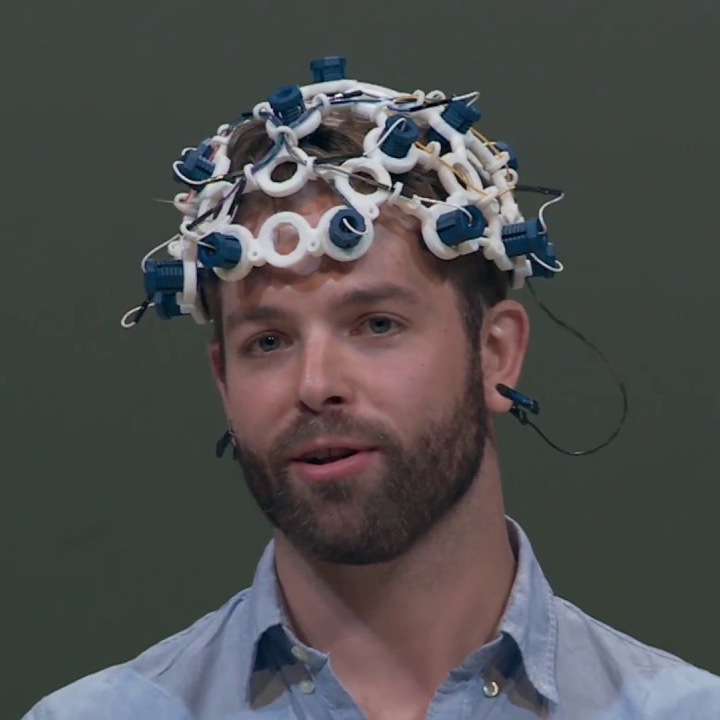
\includegraphics[width=\linewidth]{openbci.jpeg}
  \caption{OpenBCI's EEG \\ device \citep{be_superhvman_conor_2017}}
  \label{fig:openbci}
  \endminipage\hfill
  \minipage{0.32\textwidth}
  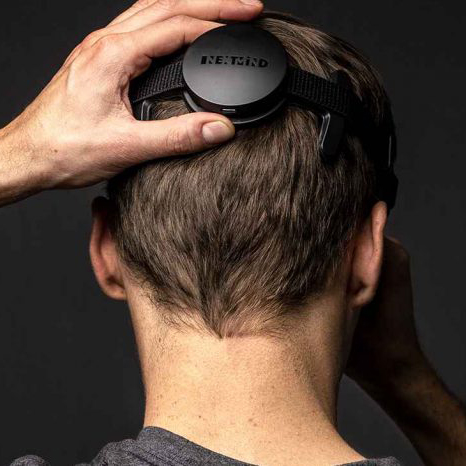
\includegraphics[width=\linewidth]{nextmind.jpeg}
  \caption{NextMind's BCI \\ device \citep{louise_neurotechnology_2019}}
  \label{fig:nextmind}
  \endminipage\hfill
  \minipage{0.32\textwidth}%
  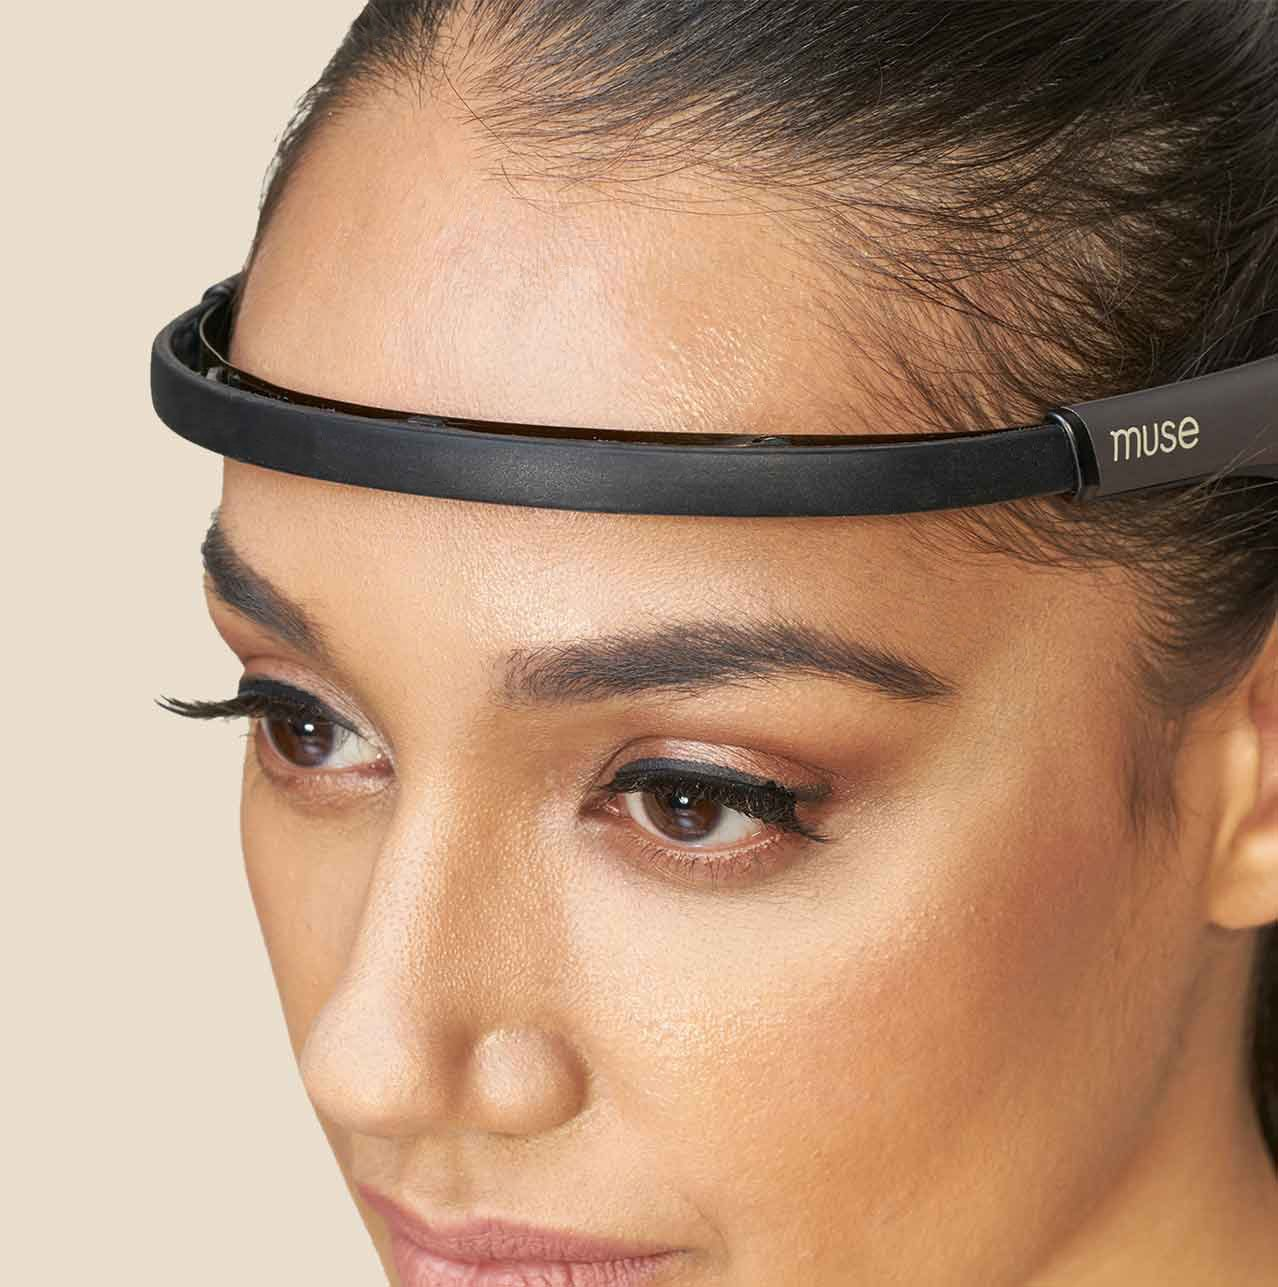
\includegraphics[width=\linewidth]{muse.jpeg}
  \caption{Muse's meditation \\ headband \citep{muse_muse_nodate}}
  \label{fig:muse}
  \endminipage
\end{figure}

A rather closed and specific BCI is, for example, the EEG headband by Muse. Its purpose is to measure meditation and sleep. They also offer an end-user app to help people better understand their meditation and sleep and how to improve them. The Muse headband is not unidirectional BCI per se, as there is also biofeedback based on neural signals, but the important difference between Muse and e.g. OpenBCI is that they abstract away the neurotechnology. Users don't need to know anything about neuroscience, neurotechnology or the interpretation and classification of brain data to get useful functionality for their use case. They also do not need to understand the software system's underlying architecture. The only thing they need to know is how to pair the device with their smartphone via Bluetooth.

Aside from full-stack BCI solutions, where a company provides a complete BCI solution including hardware and software, there are also companies that focus solely on the software aspect of neural data. Neuromore, a company based in Florida and Germany that provides a software platform for everything related to neural signal processing and BCI, is one example. The company is hardware agnostic, which means you can plug any hardware or sensor into your computer and connect it to the Neuromore Studio software. Neuromore Studio is free and open-source software that runs locally on a variety of platforms, including Windows and macOS. It provides a variety of drag-and-drop interfaces for creating and managing signal processing pipelines, even including machine learning classifiers. For example, you can transform EEG data to extract band power and create triggers based on band power selection, and generate conditional outputs for a game to e.g. move a character.

\begin{figure}[ht]
  \centering
  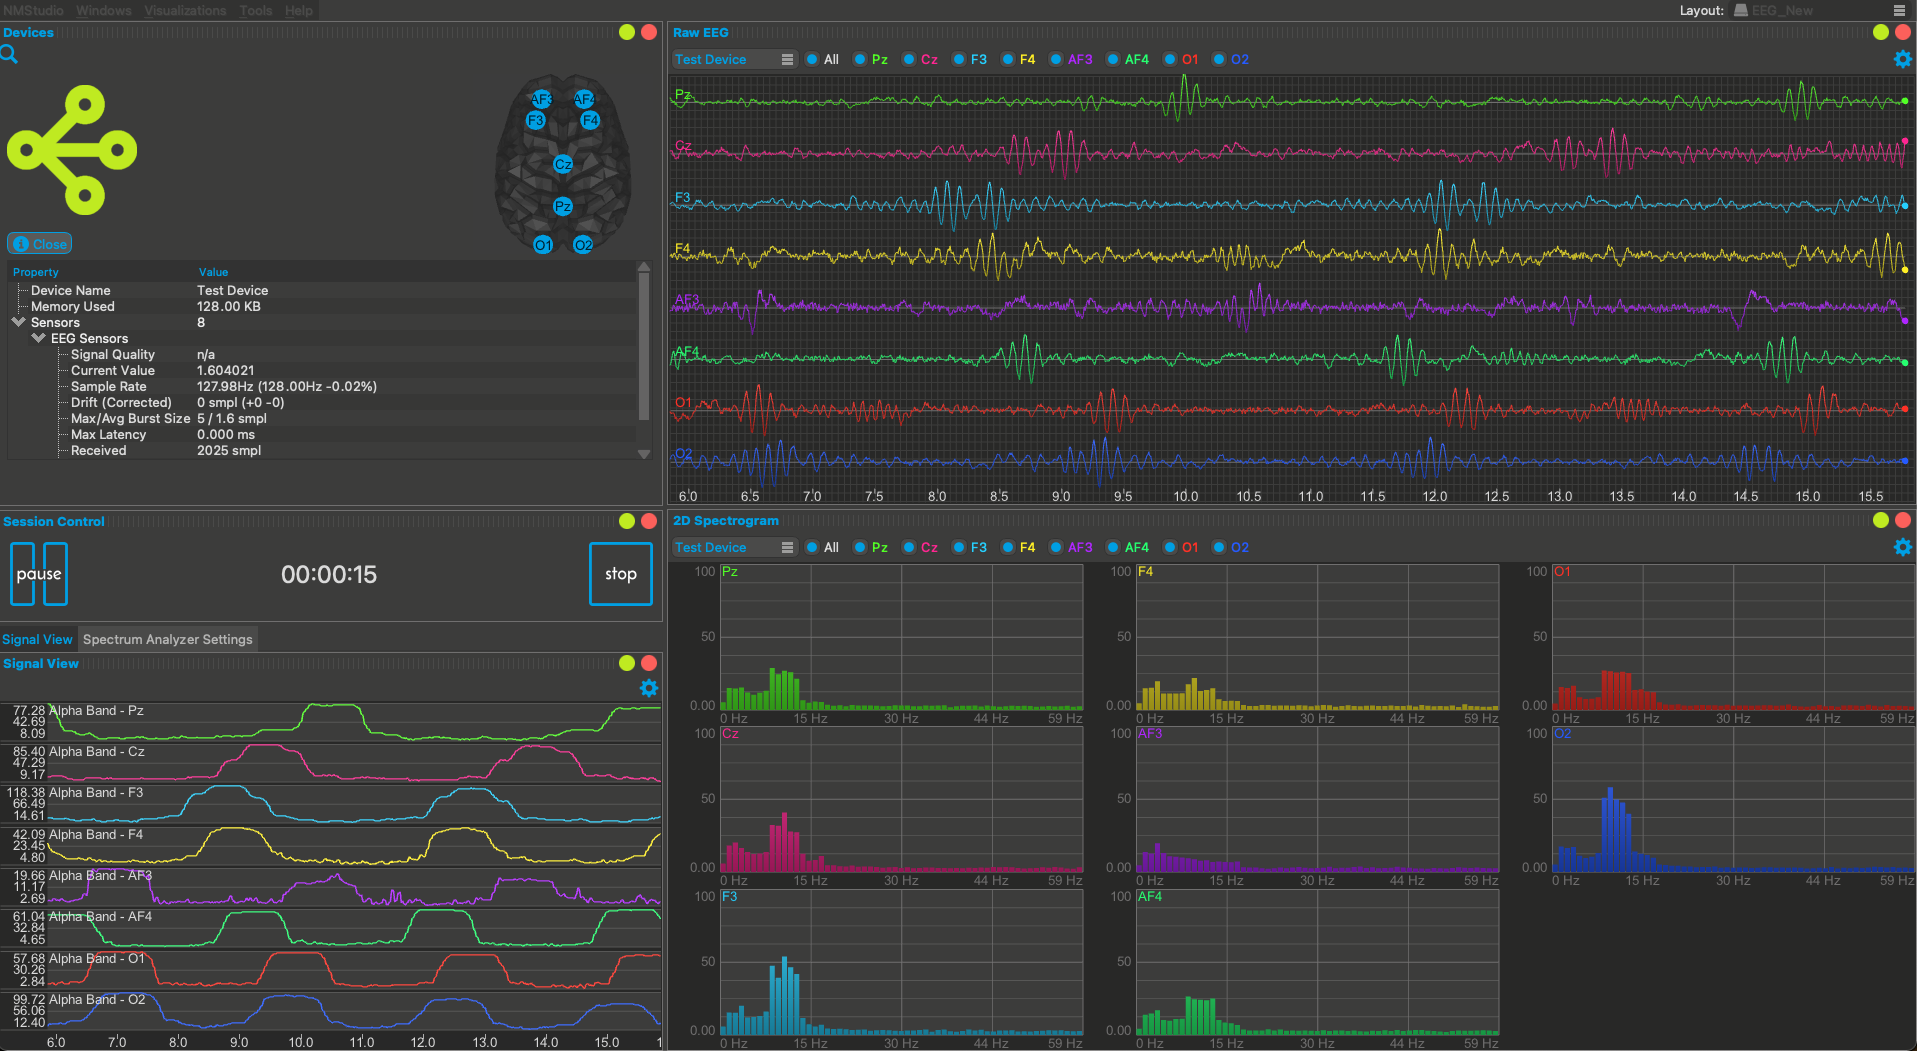
\includegraphics[width=\linewidth]{neuromore.png}
  \caption{Screenshot of the Neuromore Studio software \citep{neuromore_neuromore_nodate}.}
  \label{fig:neuromore}
\end{figure}

The author attempts to differentiate the offerings of the consumer-oriented BCIs mentioned: They either provide the hardware (with software that at least connects to the device) but are then more broadly applicable to use cases not defined by the company behind the BCI, such as OpenBCI, or they are application-specific in terms of both the software and the hardware, such as the Muse headband\footnote{Third-party developers have reverse engineered the Bluetooth features to access Muse's raw EEG data and turn it into a general-purpose device.}.

Despite the fact that this paper focuses on consumer-oriented BCIs, the applications of various BCI offerings can still be distinguished based on whether they are more consumer-oriented or research-oriented, such as the distinction between e.g. NeuroSky\footnote{NeuroSky website: https://neurosky.com} for hobbyists and Emotiv's\footnote{Emotiv website: https://emotiv.com} EEG systems, which are more research-oriented.

However, both NeuroSky and Emotiv provide a research version as well as a consumer or enterprise version of their software and hardware, aiming for general-purpose applicability across customer segments and use cases.

Other considerations include whether the applications are rather steady state evoked such as based on a frequency of noise laid on top of virtual objects to detect which object the person is looking at (e.g. as NextMind is doing), or whether they track the totality of mental states without evoking neural signals with external stimuli, such as in tracking sleep or concentration levels, both of which arise primarily evoked from inside the mind. This distinction can be made as passive, active or reactive BCI, as \citeauthor{alimardani_passive_2020} coined in their work on passive BCIs \citep{alimardani_passive_2020}. However, we do not want to include this dimension because it would introduce unnecessary and additional complexities that are more related to the application layer of BCI software.

\begin{figure}[!ht]
  \centering
  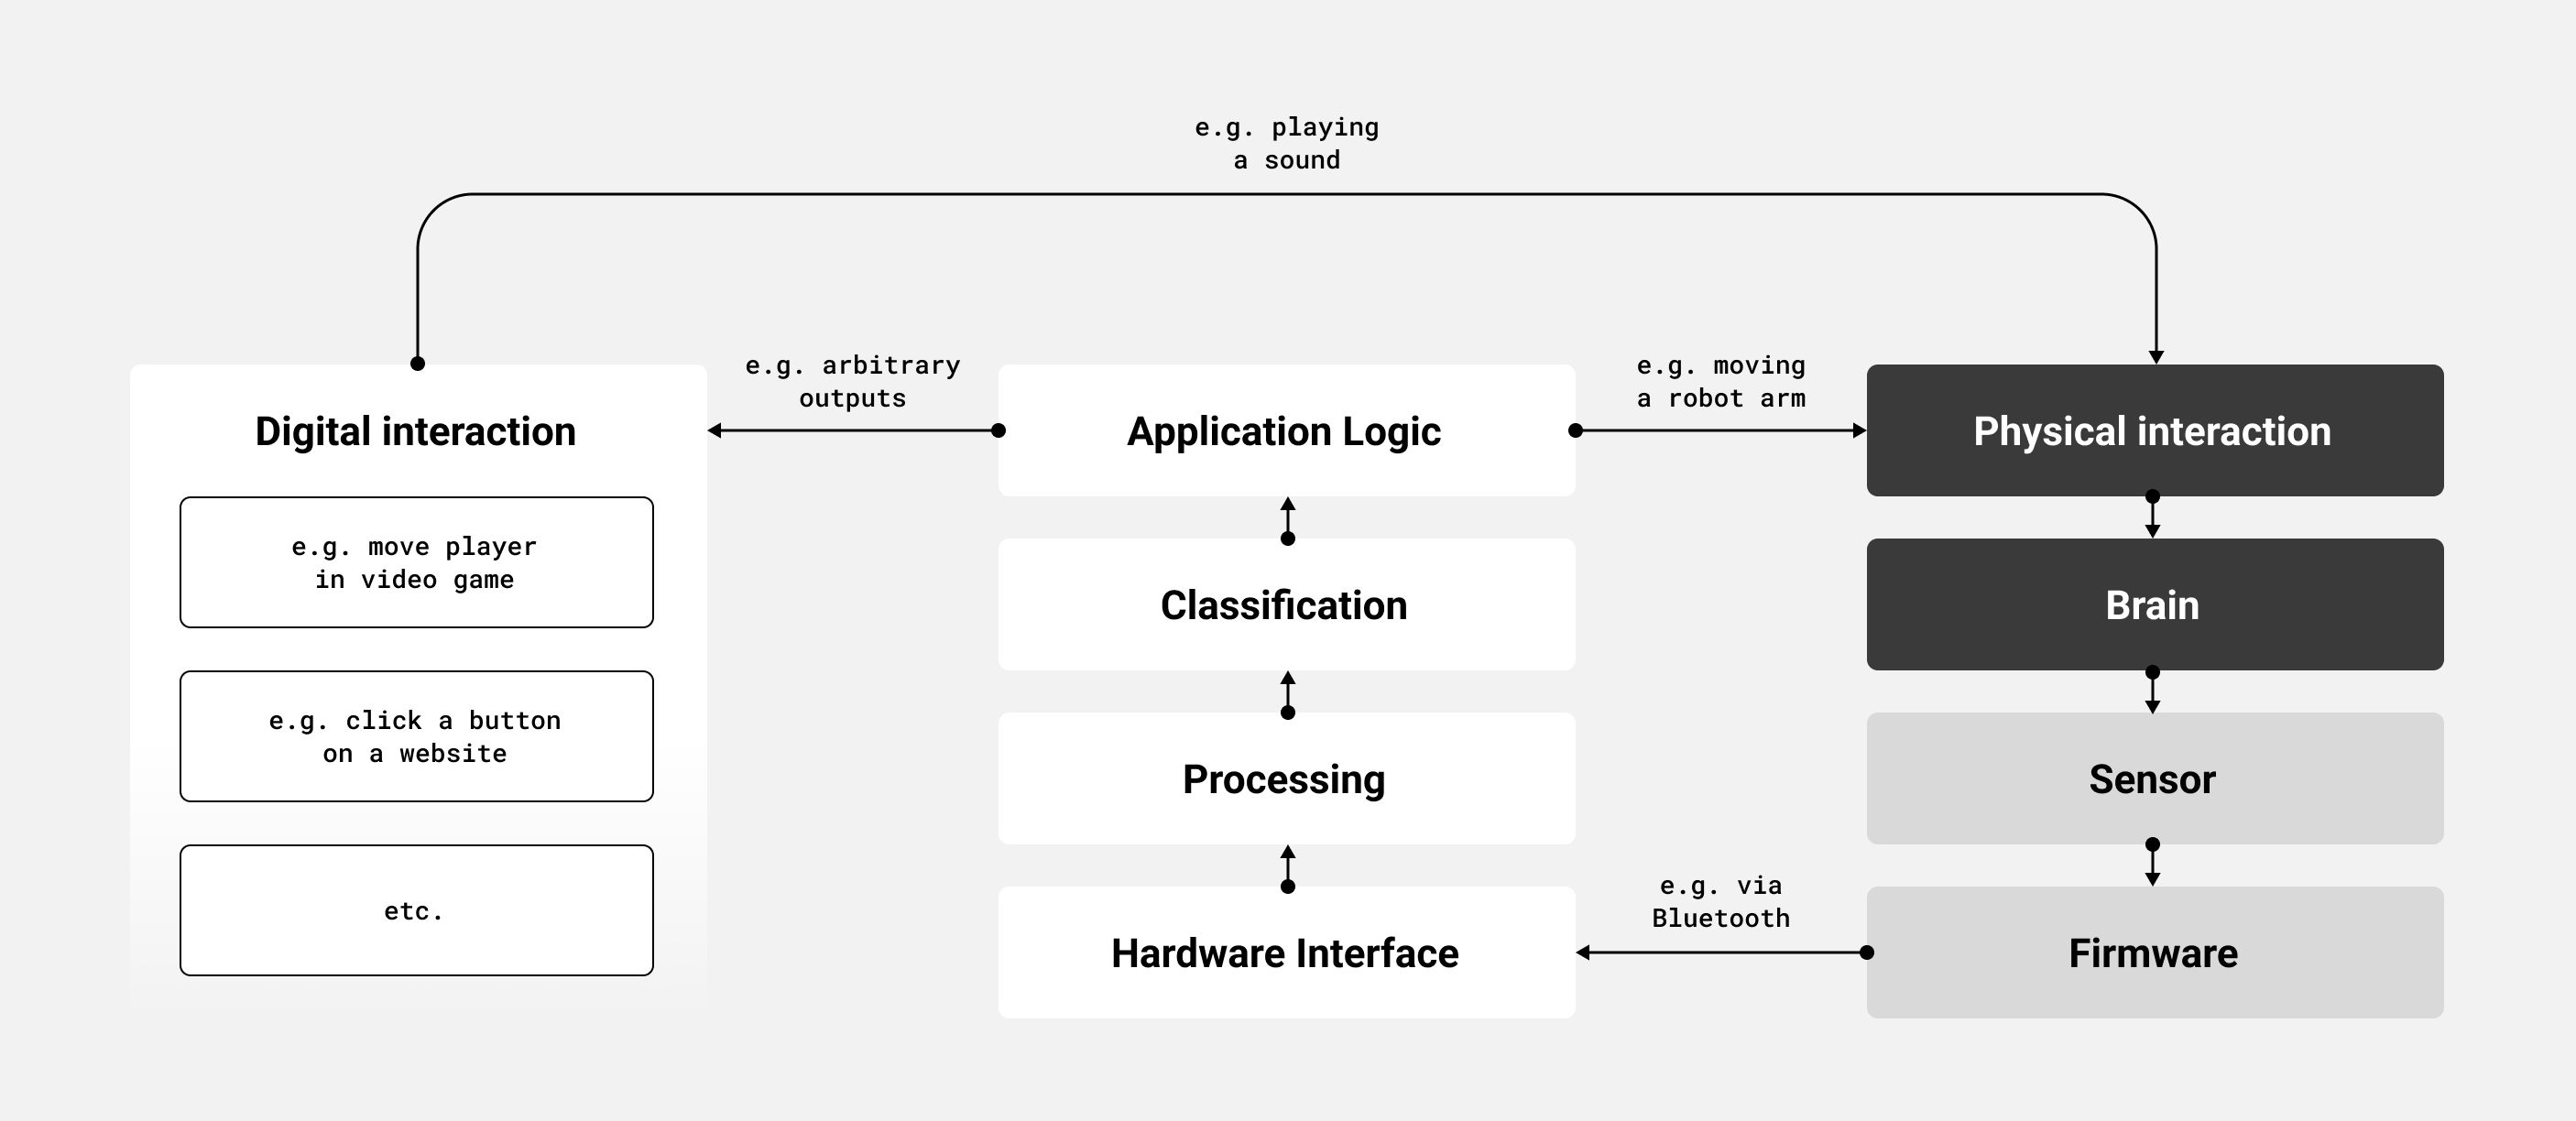
\includegraphics[width=\linewidth]{bci-components.png}
  \caption{Architectural overview of BCI components including a bidirectionality due to neurofeedback in form of e.g. playing a sound in a certain frequency to enable SSVEP (own representation, 2022).}
  \label{fig:bci-components}
\end{figure}

As shown on \autoref{fig:bci-components} there are two main components of a BCI: the hardware and the software. Next to the hardware, there is also the physical part of it, e.g. the brain and a physical interaction counterpart in form of e.g. a robot arm\footnote{Some people call this a brain-machine interface rather than a brain-computer interface because you interface with a machine rather than a computer.}. The software is the part that is responsible for the actual processing of the data, e.g. extracting the relevant information from the raw data and turning it into a meaningful output that the application layer can use. The application layer interacts then with a physical or digital counterpart to e.g. move a player in a game or turn start playing sound on the computer via its speakers.

\subsection{Unobtrusive hardware and software}
\label{chapter2-unobtrusive-hardware-and-software}

The unobtrusiveness of hardware and software is another aspect to consider when talking about BCIs. Unobtrusiveness in hardware means that it is either not visible at all\footnote{There are other things related to the overall user experience (UX) that are sometimes included in the notion of unobtrusiveness, such as comfort, reusability and convenience, where the author only implies the physical characteristics such as shape, size, etc.}, such as when sensors are implanted beneath the skull, or that it is in a form factor that is already socially accepted, such as glasses or headphones. The prototype of IDUN Technologies' hardware, which measures brain activity in the ear canal, is shown in \autoref{fig:unobstrusive-hardware} that aims to resemble in-earbuds. \autoref{fig:obstrusive-hardware} shows the Neurosity device, which measures brain activity on the head and is not comparable to a socially established form factor. What is considered socially established and accepted truly depends on the society and context, as one could argue that wearing a Neurosity device under a hat while talking to a friend is more acceptable than wearing in-earbuds. However, if, for example, in-ear EEG technology is becoming more discreet, such as hearing aids, it is more inconspicuous and socially acceptable.

\begin{figure}[!htb]
  \minipage{0.49\textwidth}
  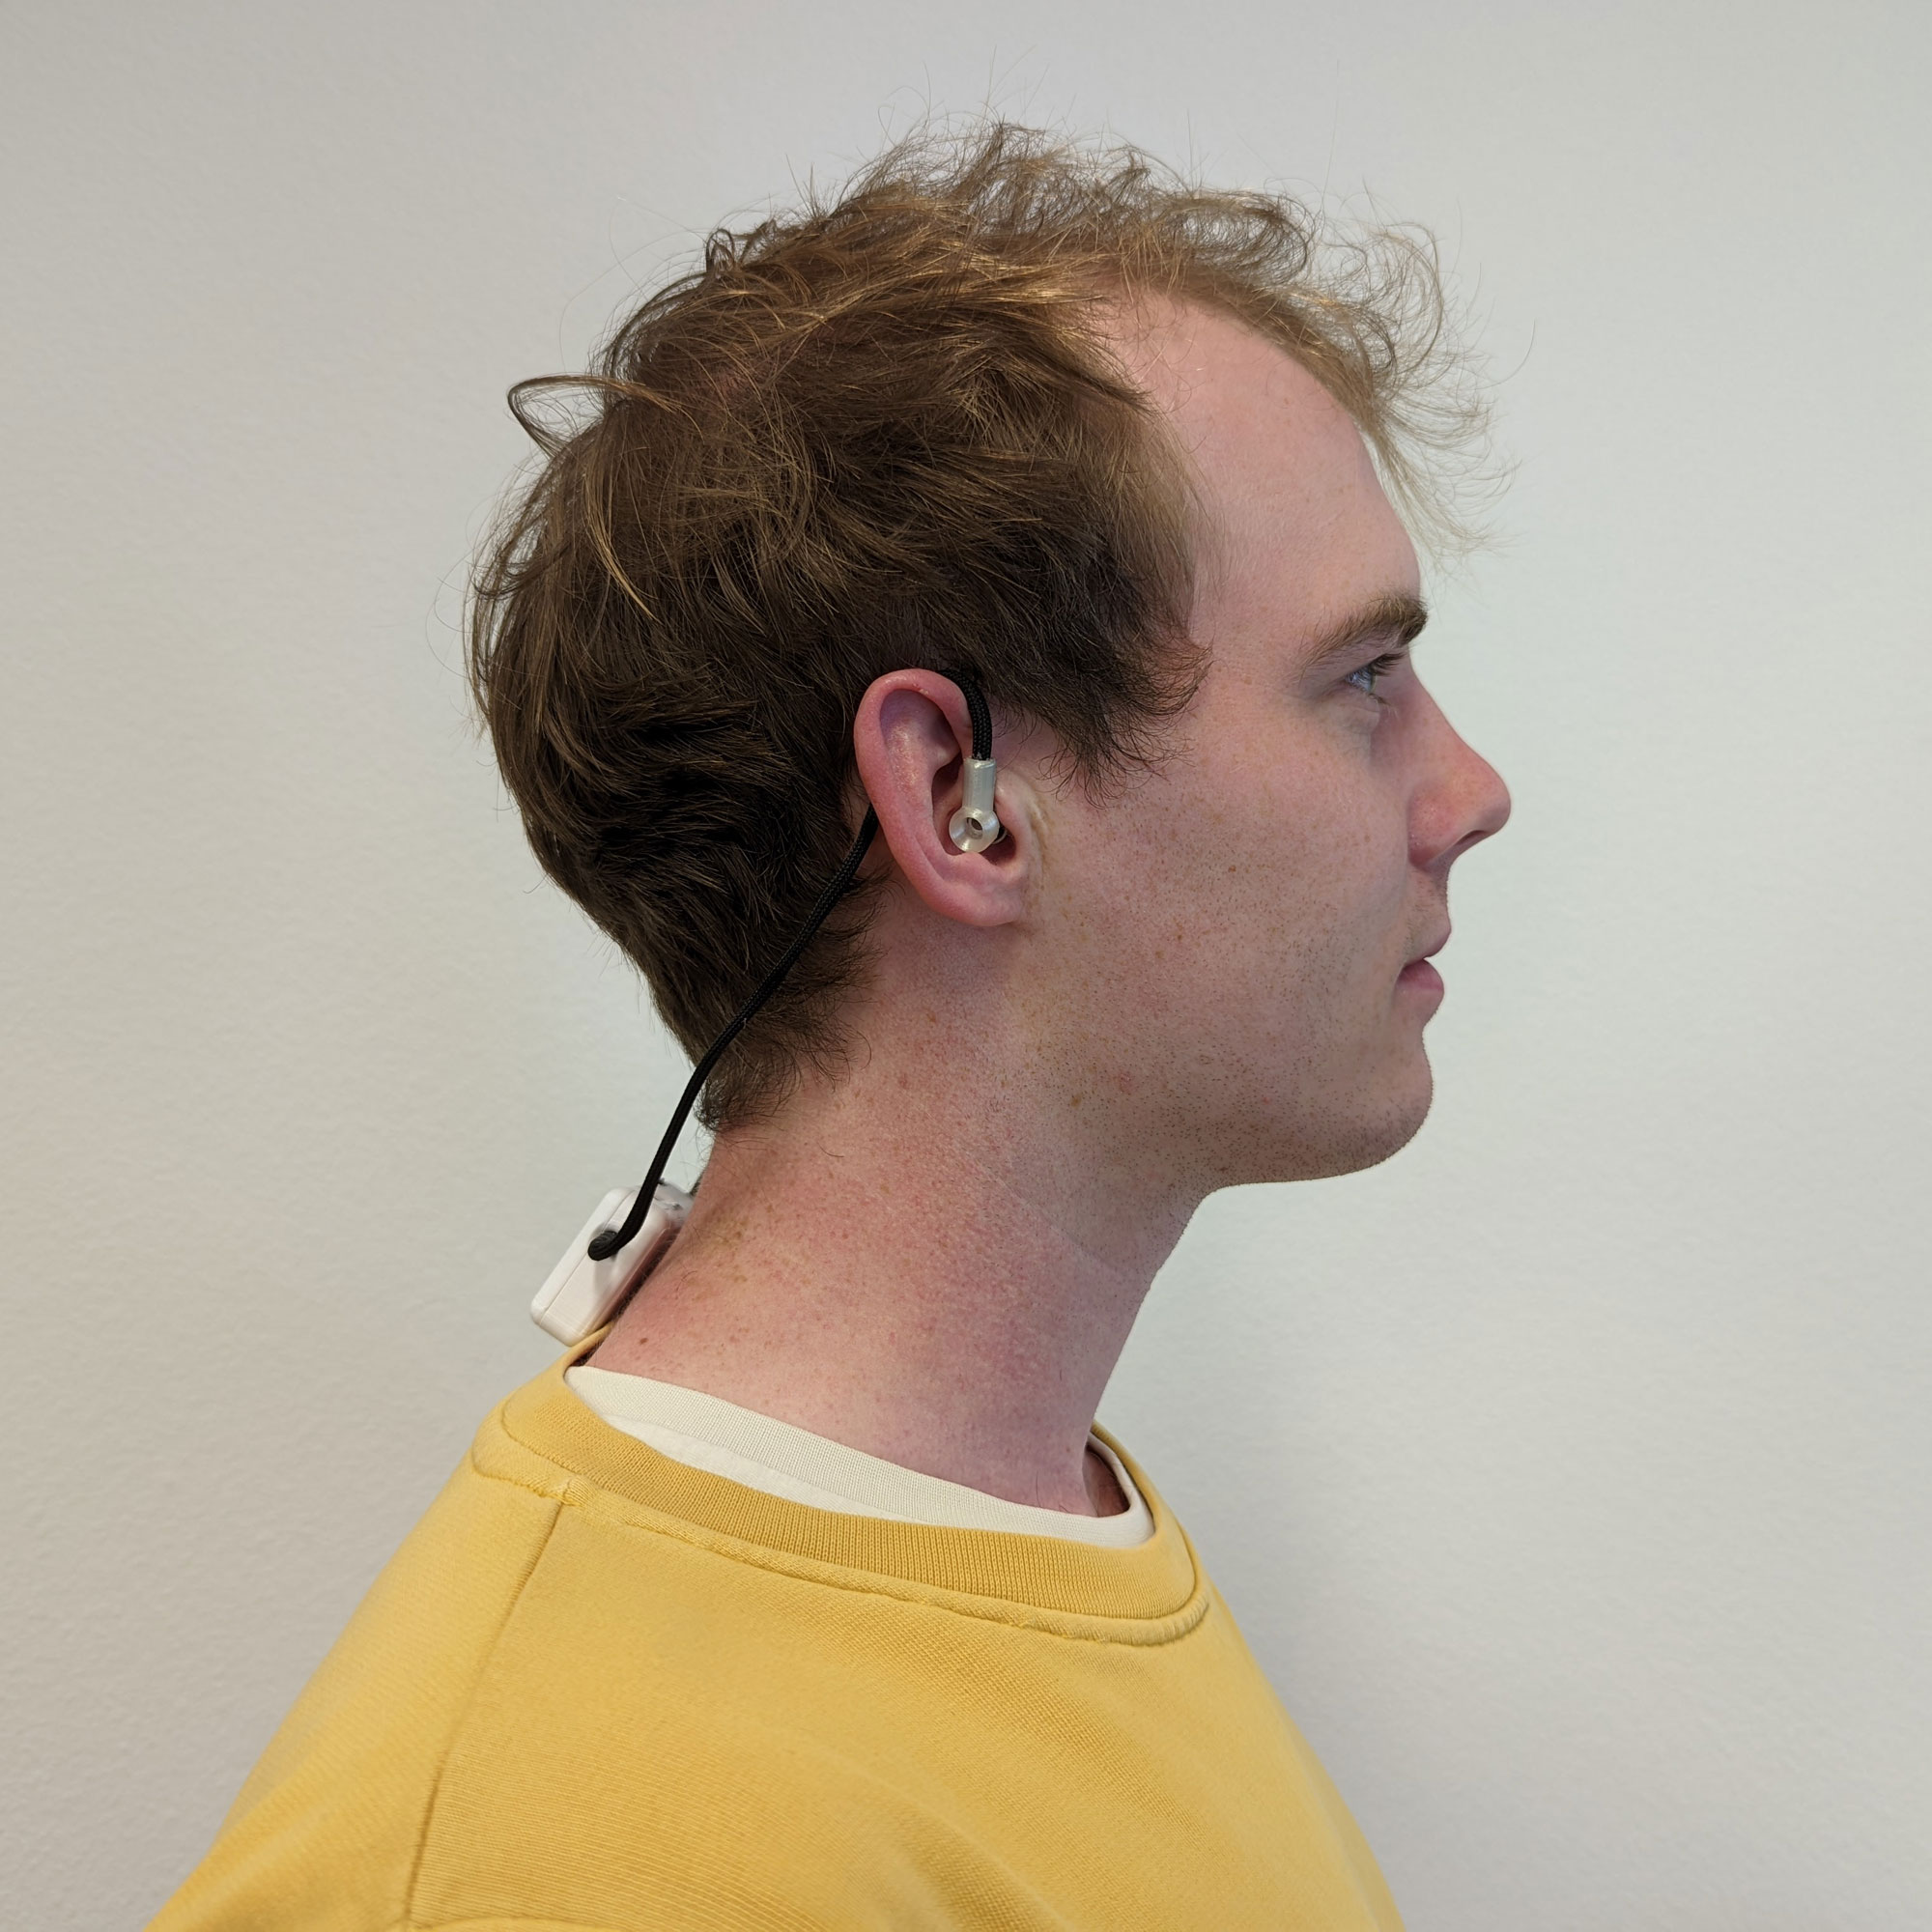
\includegraphics[width=\linewidth]{unobtrusive.jpg}
  \caption{IDUN Guardian hardware, \\ unobtrusive BCI (own representation, 2022).}
  \label{fig:unobstrusive-hardware}
  \endminipage\hfill
  \minipage{0.49\textwidth}
  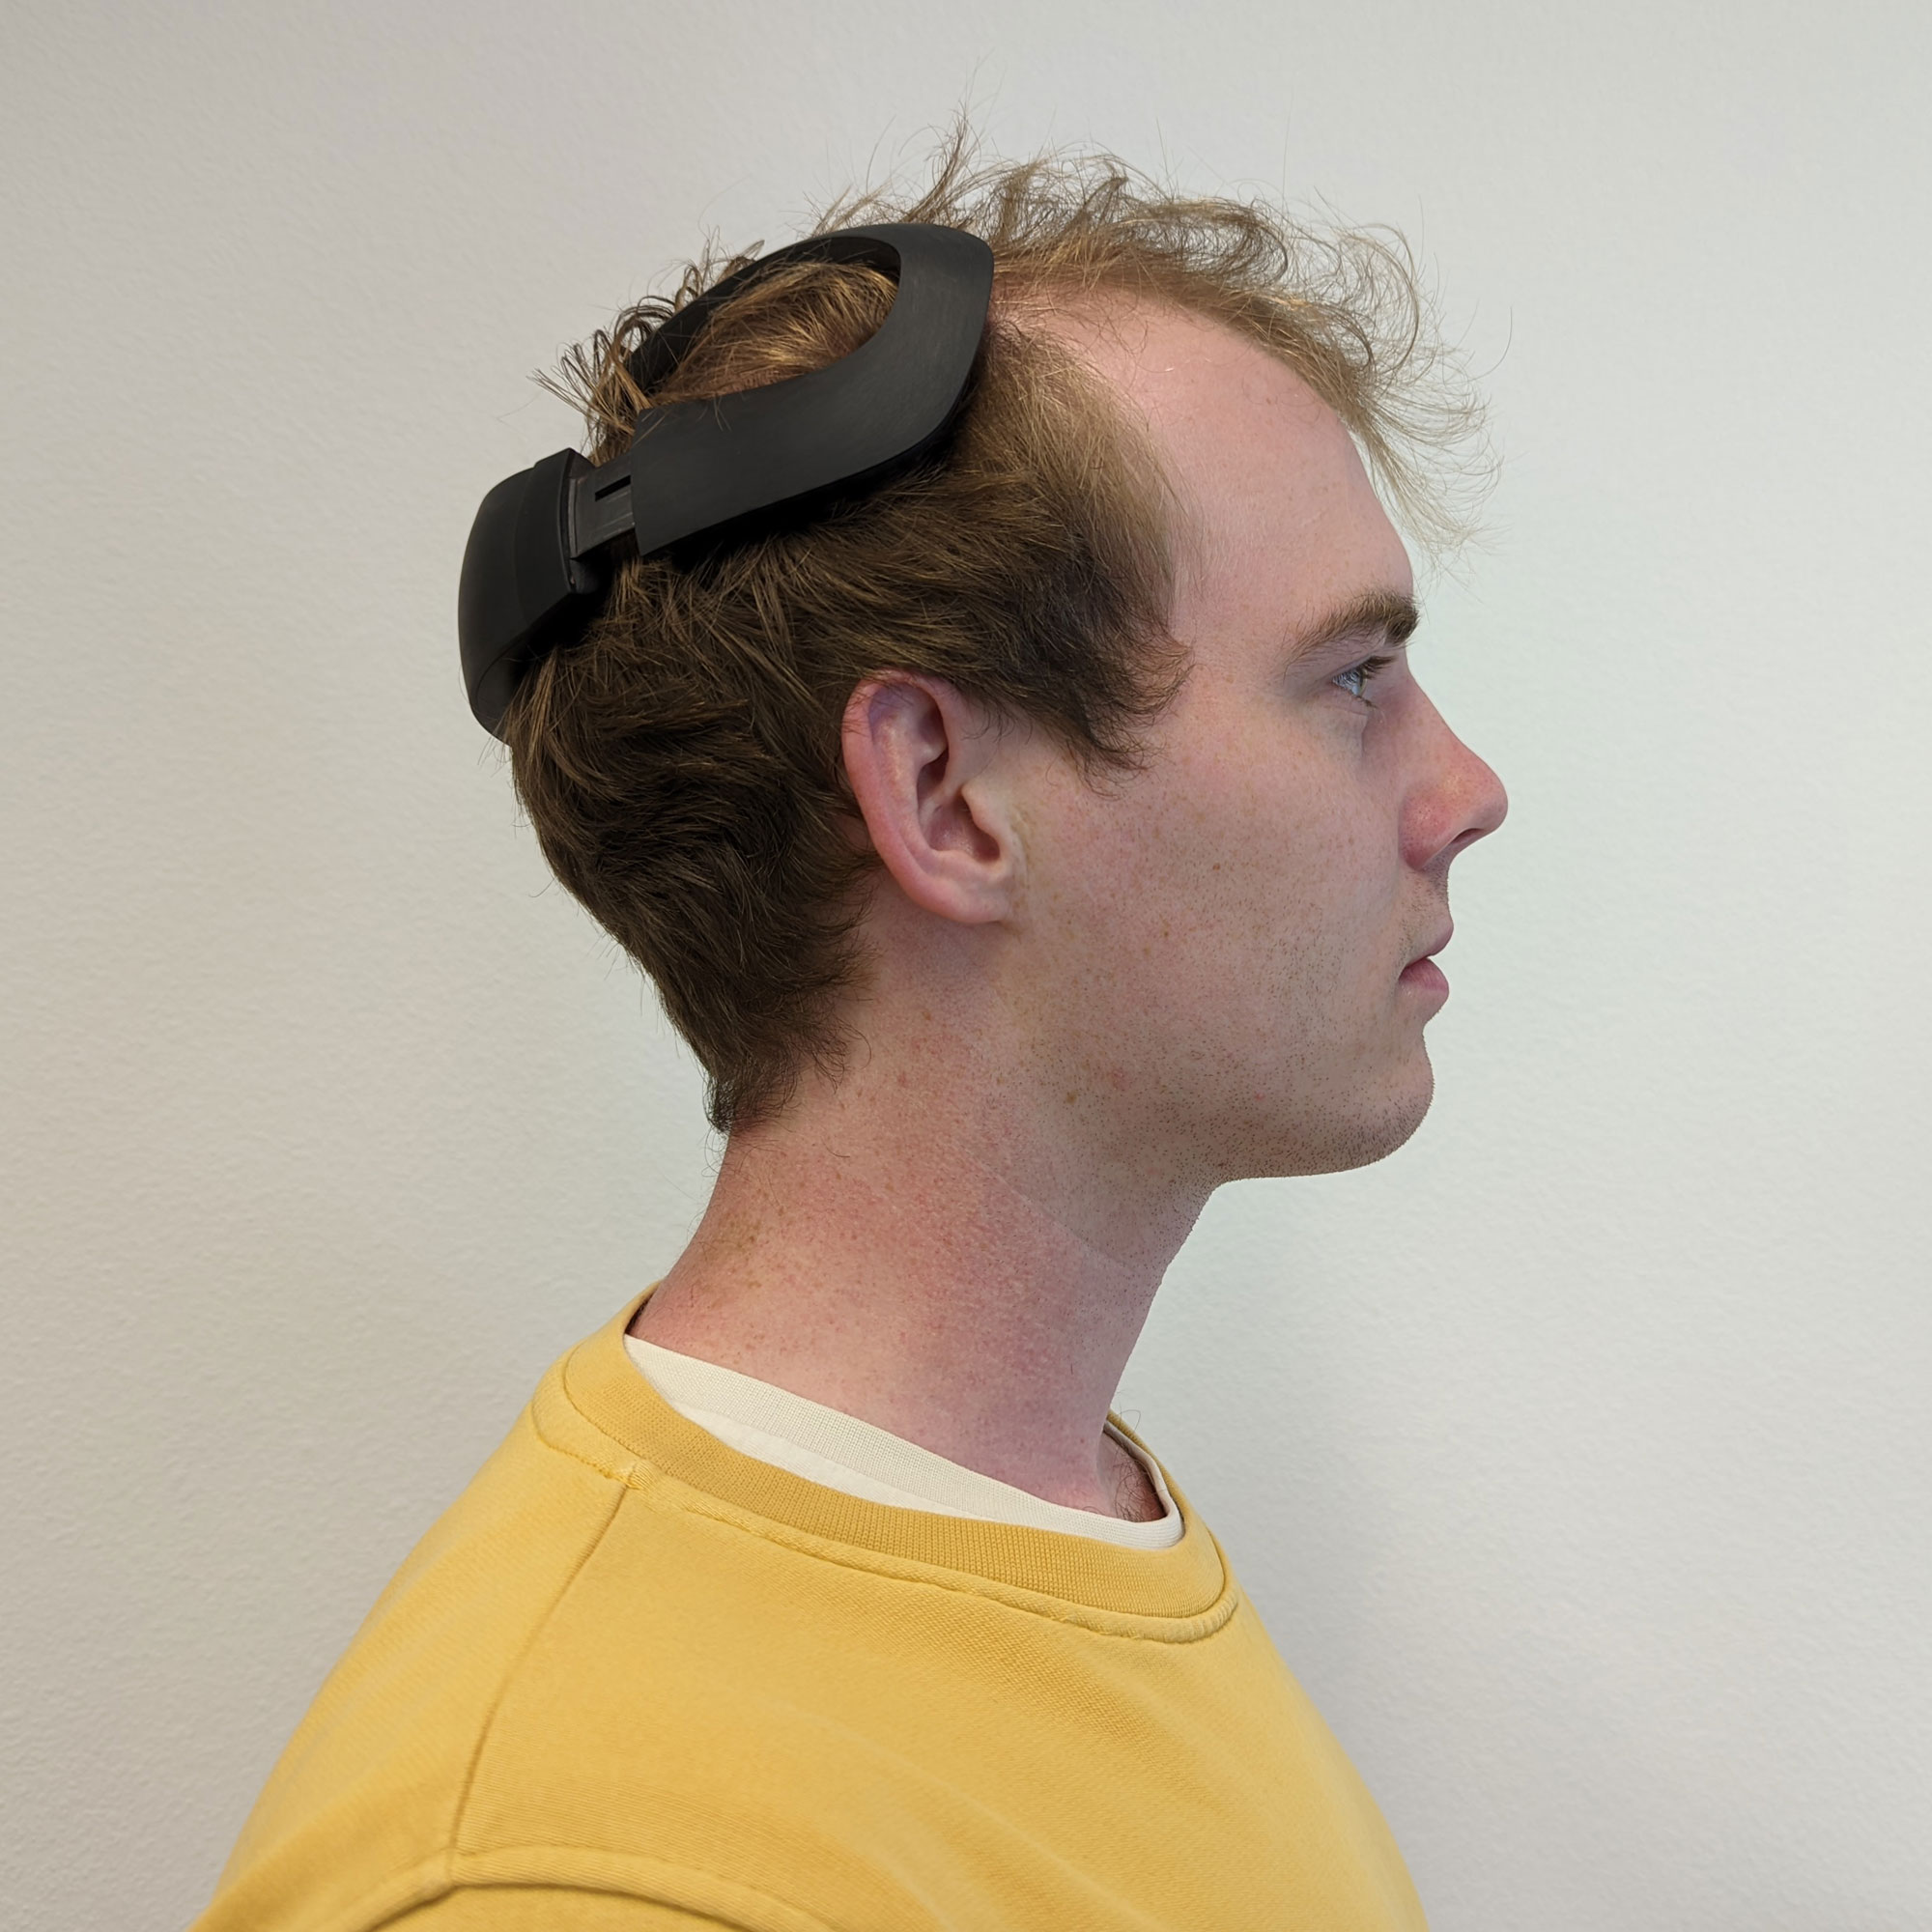
\includegraphics[width=\linewidth]{obtrusive.jpg}
  \caption{Neurosity Notion hardware, \\ obtrusive BCI (own representation, 2022).}
  \label{fig:obstrusive-hardware}
  \endminipage\hfill
\end{figure}

The implications of different form factors must also be considered, such as the possibility of moving the device and thus creating motion artefacts in the signals or the position of the sensors. The ear canal, for example, is ideally closely located to the auditory cortex of the brain but not so much for the visual cortex, which is located at the back of the head. However, further hardware implications for BCIs are not a topic covered in this thesis.

It is perhaps not as simple to discuss the unobtrusiveness of software as it is with hardware. Unobtrusive\footnote{Other words for unobtrusive could be discreet, fully-integrated, invisible or simply "in the background".} software, as defined by the author, is the abstraction of the underlying software or system that executes the logic to fulfill a task without the user knowing what the technical requirements are. As an example: To use an HP ENVY Photo 6200 printer with your Android phone, you must first download the HP Smart app and the HP Print Service Plugin app that acts as a driver for the printer in order to get it set up and running \citep{hp_hp_nodate}. In the case of the HP printer, the user must understand some of the underlying technical requirements in order for it to work, rather than simply concentrating on the task to print something. For example, unobtrusive software is when you get a new computer mouse that you simply plug in and it works\footnote{Unobtrusiveness usually correlates with usability, but it is not always the case as e.g. more advanced users wouldn't consider locked-in abstraction as more usable, therefore the aspect of usability (as well as accessibility) always remains context-bound.}.

Unobtrusive software in BCI refers to the ability to connect your hardware to your computer or smartphone and use it without the need for additional software such as drivers or command-line interface (CLI) software. As an example: To use an OpenBCI device, one needs to open the GUI app, connect the hardware, test it's quality, begin a data stream session, output the stream as e.g. a Lab Streaming Layer (LSL) or via the User Datagram Protocol (UDP), connect to the signal from e.g. Neuromore Studio \citep{openbci_neuromore_nodate}, run the data through a classification pipeline, and then connect the output from Neuromore to a video game via the engine itself to have controls for the video game. It should go without saying that this is not unobtrusive software.

There are examples of software that is included as an executable file and thus is rather unobtrusive, but the software is closely linked with the hardware and the brand behind the hardware, or it is in the proof of concept (PoC) stage rather than a production-ready application. Buying a new pair of headphones and plugging them into your computer to enjoy neuro-enhanced experiences that interact with your brain's outputs or measure brain data across all apps, the operating system, and so on would be an example of completely unobtrusive software. One step into this direction would mean to create standards such as a common understanding of a N/CI or in general to come out of the PoC stage of most BCI software and rather create extensible and production-ready software.

\newpage
\subsection{Production-grade software}
\label{chapter2-production-grade-software}

There is no textbook definition of what production-grade software is, but in most cases, software developers agree on the following points:

\begin{itemize}
  \item The software works at any time when access is required. It is therefore capable for frequent and intensive use in commercial or industrial environments.
  \item Software whose behaviour is deterministic and predictable and which is therefore well-tested, well-documented and optimised in terms of speed, efficiency and security for the given context (e.g. the size of the user base). Usually developers agree on a Definition of Done (DoD) inside their team to what is considered production-ready, e.g. including a test-coverage of 80+\%, peer-reviewed and commented code, common code style guide etc.
  \item Software that runs in a production environment, i.e. on a cloud computing cluster for actual users rather than in a test environment with test users or, for example, on hardware delivered to real customers, and that is able to adapt itself to the context, e.g. to a higher access rate or insecure user-generated input. In most cases, especially in cloud computing, production-ready also means larger data sets, such as in databases, the possibility of a greater number of edge cases due to a larger user base, and, most importantly, more available computing power on production instances.
\end{itemize}

As stated in previous sections, most BCIs, such as the OpenBCI, are not intended for production. They are intended for PoCs that are used in examples, such as controlling objects in games or conducting research. End-to-end and full-stack BCIs for production are rare, as most are very specific and not intended for general purposes, such as the Muse headband, or the software aspect is intended for PoCs or researchers, such as with Emotiv. Pure software products, such as Neuromore, lack the hardware component and miss, for example, an SDK that can be integrated into existing software for different platforms. Neurosity, for example, the company behind the device depicted in \autoref{fig:obstrusive-hardware}, aims to provide a universally usable and unobtrusive software stack that is even open-source. However, because the hardware isn't unobtrusive enough, it doesn't qualify the author's definition as production-ready (apart from the fact that it is not known whether their software stack is actually aimed to be used in production \citep{neurosity_neurosity_2022} or that third-party developers provide disclaimers of being a work in progress \citep{turney_notion_2022}).

\newpage

Companies such as e.g. Neuralink are presumably working on a general purpose, unobtrusive and production-ready software system which enables developers to build production apps and even platforms on top of it for a variety of use cases without being limited \citep{musk_integrated_2019}, in their case, since it is a bidirectional BCI, developers are also able to write data back to the brain. Since their aimed hardware is also as unobtrusive in the form factor (since it's implanted) they have a high potential to become one of the first mass-market ready BCIs if we ignore the fact that we need a surgery to get the device itself \citep{neuralink_approach_nodate} and other considerations as a harder opt-out of the device compared to e.g. plugging out earphones.

\section{Neural/cloud interface definition}
\label{chapter2-neural-cloud-interface-definition}

This section discusses the definition, need and differentiation of a N/CI and the paradigm shifts associated with it when talking about BCI software.

\subsection{BCI software on the cloud}
\label{chapter2-bci-software-on-the-cloud}

Having a look at \autoref{fig:nci-components} we can see that the three software layers of a BCI-component illustration as pictured on \autoref{fig:bci-components} is highlighted. This is due to the fact that these components are able to run on the cloud, i.e. on a public cloud provider such as Amazon Web Services (AWS).

\begin{figure}[!ht]
  \centering
  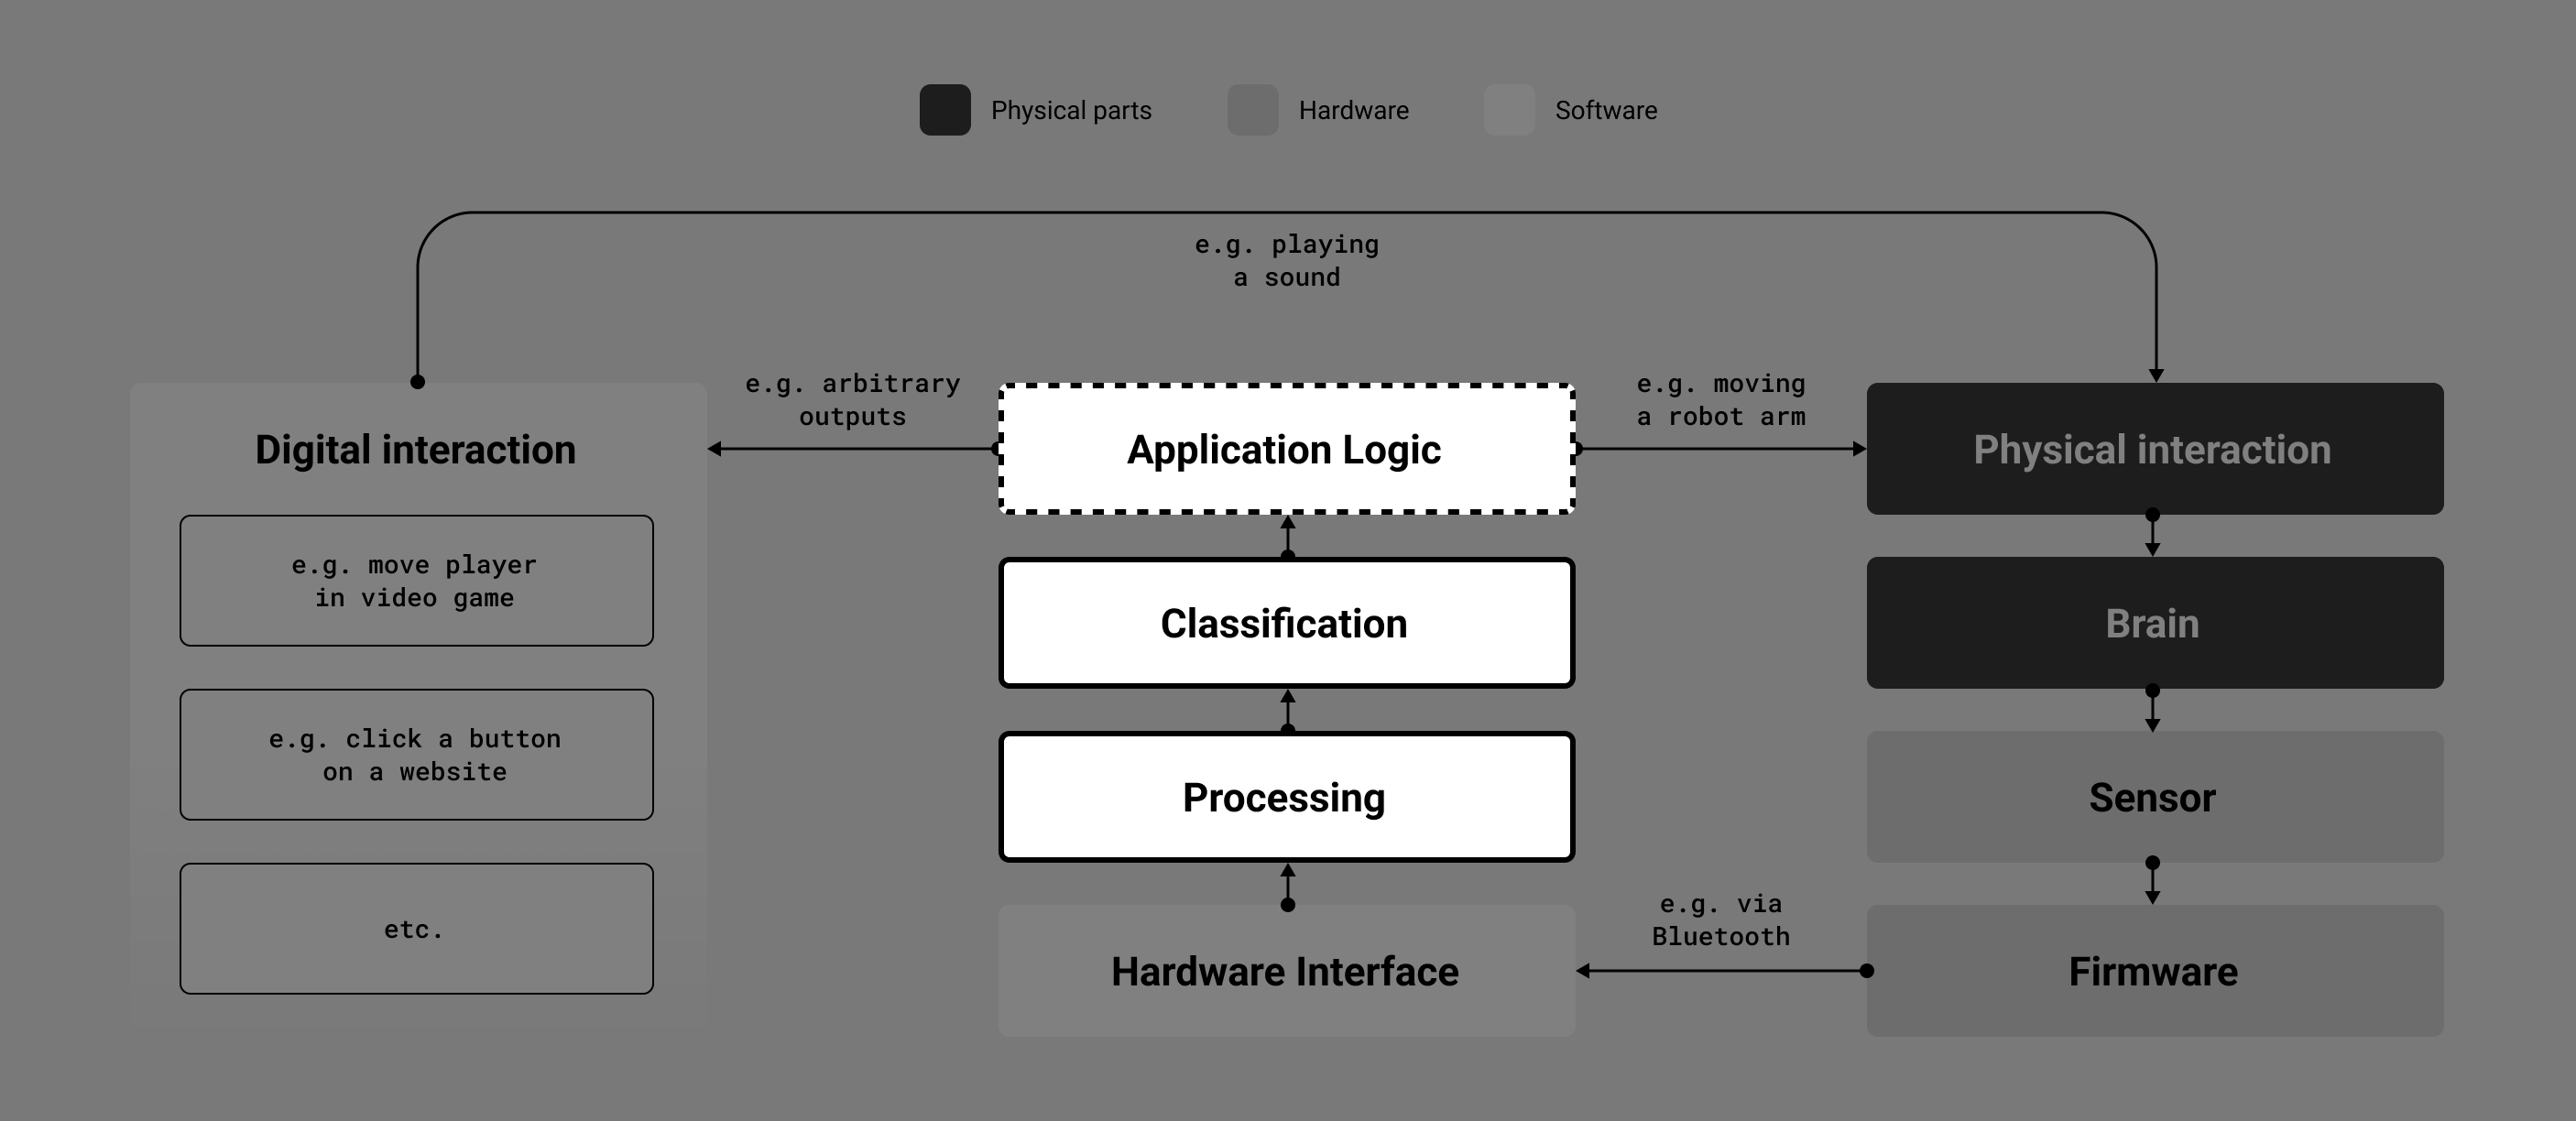
\includegraphics[width=\linewidth]{nci-components.png}
  \caption{Highlight of the software components as shown on \autoref{fig:bci-components} of a BCI that could be moved to the cloud. The Application Logic layer can partially be part of the cloud, but doesn't need to be entirely part if it (own representation, 2022).}
  \label{fig:nci-components}
\end{figure}

Running software on the cloud means that developers or companies can access provisioned information technology (IT) infrastructure through the internet usually with a pay-as-you-go pricing model \citep{amazon_web_services_inc_what_nodate}. Development speed of software applications can drastically improve since software developers can only focus on software, rather than incorporating the hardware and network aspect of setting up their own server farms, therefore abstracting the hardware part away. What started out with simple computers that can be rented on a server such as it was with e.g. AWS Elastic Compute Cloud (EC2) \citep{barr_amazon_2006} ended up being a diverse offering from cloud providers offering various levels of abstracted offerings as shown on \autoref{tab:cloud-computing-types}.

\begin{table}[!ht]
  \centering
  \resizebox{\textwidth}{!}{%
    \begin{tabular}{ll}
      \rowcolor[HTML]{000000}
      {\color[HTML]{FFFFFF} Type}                                                                                 &
      {\color[HTML]{FFFFFF} Description}                                                                                                                                                                                                                                                                                                                           \\ \hline
      \multicolumn{1}{|l|}{\textbf{\begin{tabular}[c]{@{}l@{}}Infrastructure as\\ a Service (laaS)\end{tabular}}} &
      \multicolumn{1}{l|}{\begin{tabular}[c]{@{}l@{}}IaaS gives access to data storage space, virtual or dedicated\\ computers, and network services. The greatest degree of\\ flexibility and administrative control over your IT resources\\ are provided by utilising IaaS.\end{tabular}}                                                                       \\ \hline
      \multicolumn{1}{|l|}{\textbf{\begin{tabular}[c]{@{}l@{}}Platform as a\\ Service (PaaS)\end{tabular}}}       &
      \multicolumn{1}{l|}{\begin{tabular}[c]{@{}l@{}}PaaS lets developers concentrate on developing and\\ managing their code rather than worrying about the\\ underlying infrastructure (often hardware and operating\\ systems). An example is Kubernetes.\end{tabular}}                                                                                         \\ \hline
      \multicolumn{1}{|l|}{\textbf{\begin{tabular}[c]{@{}l@{}}Software as a\\ Service (SaaS)\end{tabular}}}       &
      \multicolumn{1}{l|}{\begin{tabular}[c]{@{}l@{}}SaaS provides a whole product that is run and controlled \\ by the service provider. The phrase SaaS often refers to\\ end-user apps (e.g. web-based email). Developers don't\\ have to be concerned about how the service is handled\\ or whether the underlying infrastructure is maintained.\end{tabular}} \\ \hline
    \end{tabular}%
  }
  \vspace{10pt}
  \caption{The three abstraction levels and types of cloud computing \citep{amazon_web_services_inc_what_nodate}.}
  \label{tab:cloud-computing-types}
\end{table}
\raggedbottom

The majority of businesses are anticipated to embrace a cloud-first strategy by 2025, according to Milind Govekar, vice president of IT research and consultancy company Gartner, and will not be able to fully implement their digital plans without the usage of cloud-native architectures and technologies \citep{gartner_gartner_nodate}. The impact and importance of cloud computing cannot be underestimated, and its success is also reflected in the annual spending on cloud computing resources, estimated at €474 billion in 2022 \citep{gartner_gartner_nodate}. Cloud computing is such an extensive and complex topic that it could easily fill entire books. In the following list, the author categorises three important points from a bird's eye view that certainly play an important role when it comes to BCI software: 1. Dedicated and deterministic environments, which explains that an environment of a software programme always stays the same independent of the end-users hardware, 2. elastic and high performance availability, which explains cloud computers that have a on-demand and adjustable high-performance and 3. provided services for speed, which explains the concept of pre-made and dedicated software written especially for the cloud and certain use cases.

\begin{itemize}
  \item \textbf{Dedicated and deterministic environments:} Running code for BCIs on different end-user platforms, such as Windows or Android, can have drawbacks because each device has its own processor, graphics card, operating system version, drivers etc., which can make developing software that requires stable and good performance, such as a neural data processing pipelines, time-consuming and difficult to maintain, as developers must keep track of every factor of the end-user devices. This is fine for BCIs that are not intended for the general public, such as specially designed BCIs for people with, say, locked-in syndrome, but for the general public, a variety of different end-user devices come into play. When code is run on a dedicated machine, such as a cloud computer with clearly defined hardware and operating system specifications, it becomes less error-prone and more deterministic. The use of virtual machines (VMs) or containerization on end-user devices attempts to solve this problem, but has additional drawbacks that are beyond the scope of this thesis. Most notable is the draw-back of being bound of the end-users device performance which also varies from user to user.
  \item \textbf{Elastic and high performance availability:} Because the cloud model usually runs as an as-needed model, the initial purchase cost of computer hardware is split and shared across usage. Developers have access to tremendous computing power that would not be easily afforded if purchased on its own. As a result, when developing a computationally intensive algorithm, developers can use high-performance central processing units (CPUs) and graphics processing units (GPUs) to complete tasks much faster than consumer hardware on end-user devices. Performance can also be increased as needed, for example, to handle heavier tasks that are not used as frequently, or to handle more requests when, for example, the demand on the software increases due to an increase in the number of users, which is a a process known as elasticity \citep{gartner_definition_nodate}. Furthermore, the cloud provides far more storage capacity than end-user devices. End-users would request more data as needed, which would then be downloaded to their device via the internet, rather than all of the data filling up their device's storage capacity.

  \item \textbf{Provided services for speed:} The vast majority of cloud providers are providing more specialised services as we move closer to PaaS. Provisioned database servers, for example, exist solely to serve as a database, so the underlying hardware is optimised for the database software running on it, such as e.g. PostgreSQL. There are hundreds of cloud computing services available, including 200 from AWS alone \citep{amazon_web_services_inc_what_nodate}, all of which address specific use cases. This is extremely useful when it comes to cloud-based BCI software. One example is the aspect of live streaming of brain data, which we will go over in greater detail in the thesis' implementation chapter. The services provided accelerate development by eliminating the need for teams to reinvent the wheel over and over again, and they also provide out-of-the scalability such as in the serverless model \citep{redhat_what_2022}.
\end{itemize}

An N/CI can use cloud computing by running certain software components of a BCI system in the cloud as e.g. shown on \autoref{fig:nci-components}. Multiple BCIs can communicate with each other or with other software or hardware over the internet, enabling remote HCI. \autoref{fig:nci-components} depicts how two or more BCIs can interface with one another using cloud software. The red arrows represent the typical BCI possibility of local HCI. The blue arrow depicts how the person on the left can execute business logic via the cloud over the internet, enabling digital and physical interactions with e.g. high performance. The green arrow depicts how the person on the right can communicate with their BCI via a N/CI with the person on the left even if they are not in the same geographical location.

\begin{figure}[!ht]
  \centering
  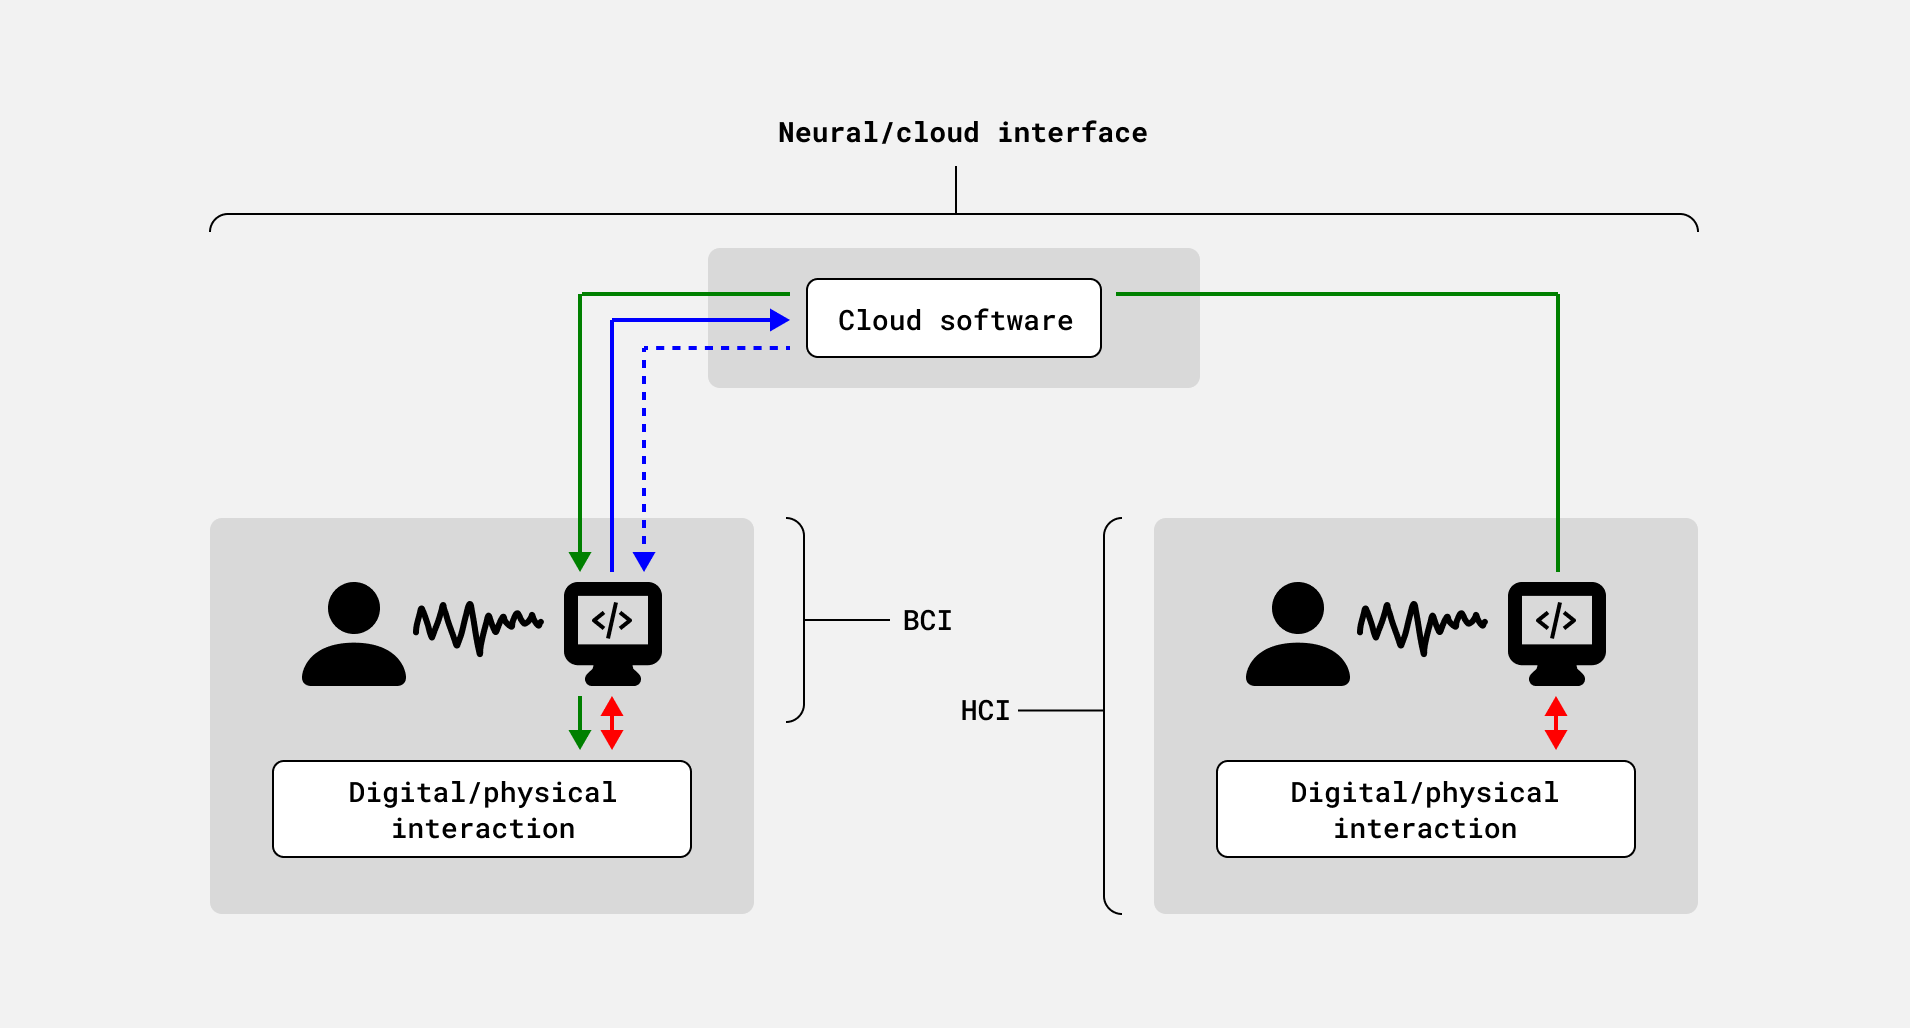
\includegraphics[width=\linewidth]{nci-overview.png}
  \caption{A N/CI is the connection between multiple BCIs (own representation, 2022).}
  \label{fig:nci-overview}
\end{figure}

\begin{figure}[!ht]
  \centering
  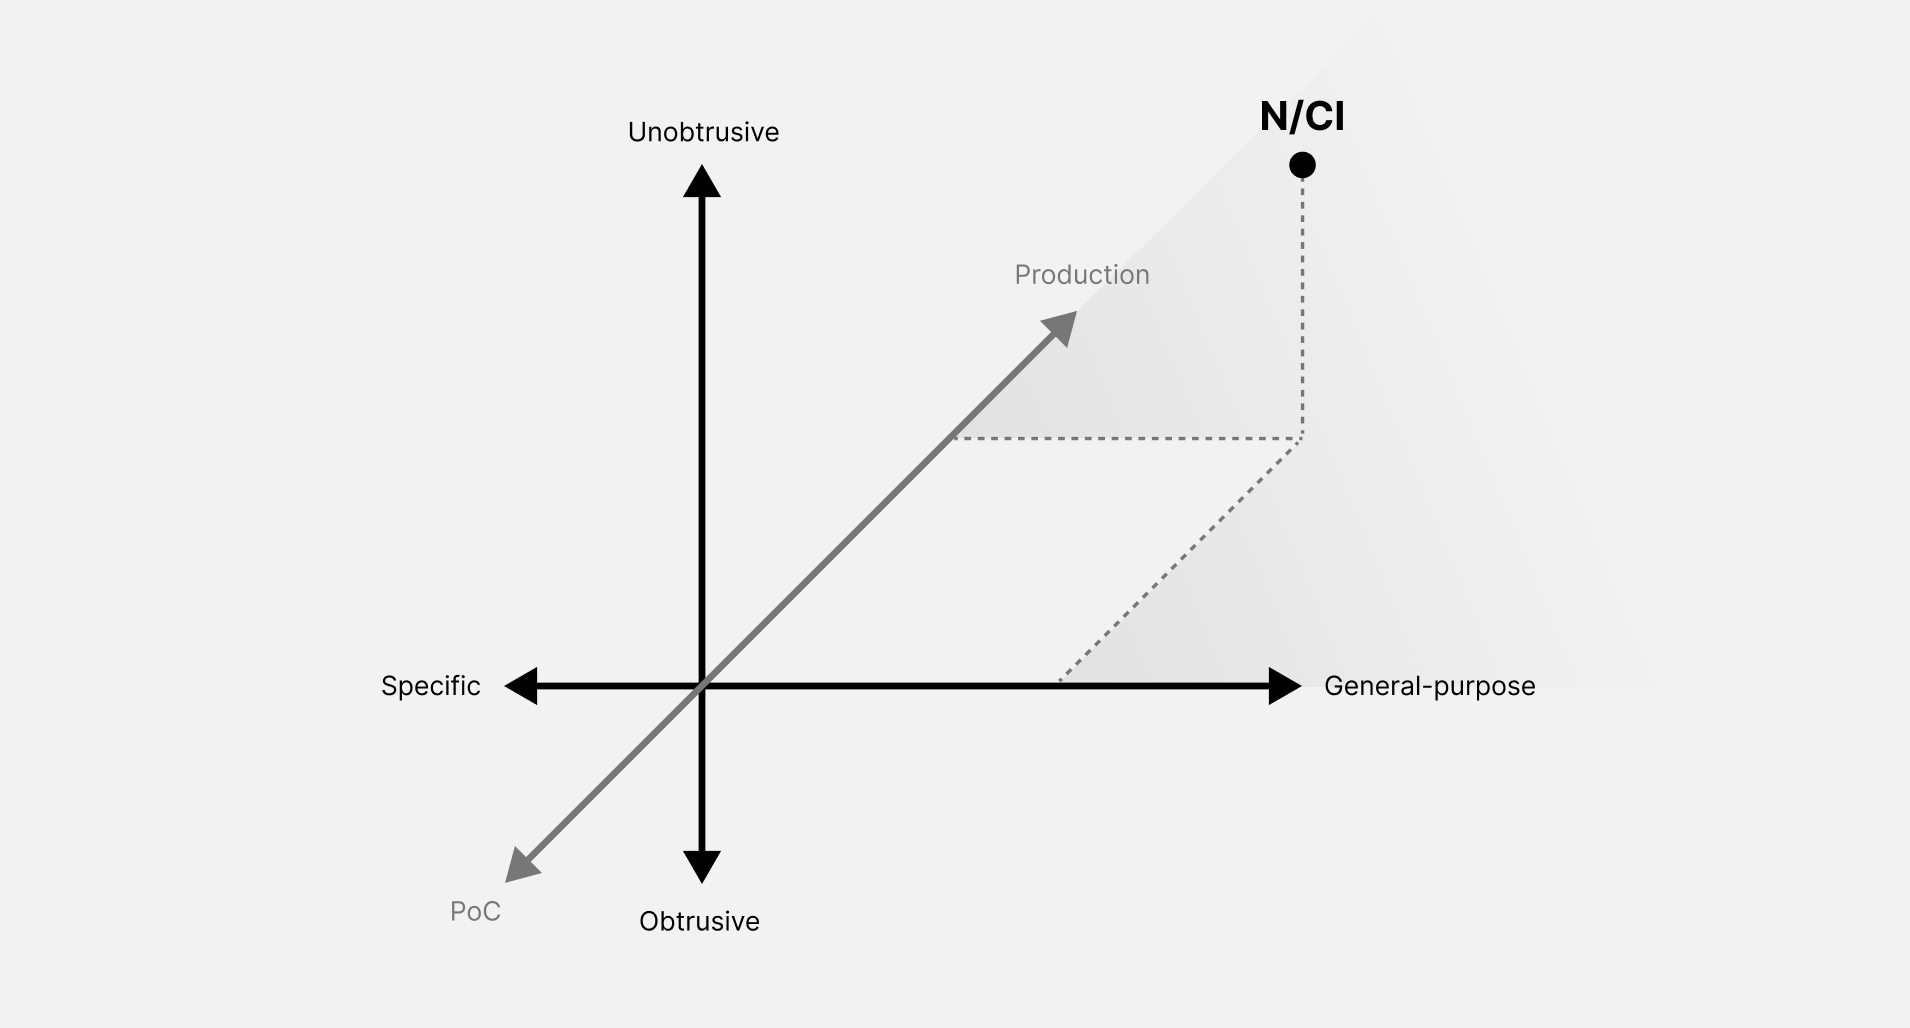
\includegraphics[width=\linewidth]{nci-definition.png}
  \caption{Visualisation of the three-dimensionality of the term neural/cloud interface (own representation, 2022).}
  \label{fig:nci-definition}
\end{figure}

\subsection{Three-dimensionality of a N/CI}
\label{chapter2-three-dimensionality-of-a-nci}

% General definition of a N/CI
% General challenges of a N/CI

% Difference between existing software systems that come close to a N/CI
% Opt-in is based on ourselves rather than an account
% Create another list with the challenges of a N/CI and use them for the solutions in the methodologies and implementation sections

% Akademischer Hintergrund: Vorbilder, Referenzmaterial, Eingrenzung und vertiefte Begründung der Zielformulierung. Grundlagenforschung im Bereich vergleichbarer Medienprodukte. Kenntnis der fachspezifischen Theorien und Techniken. Hier muss umfassende Fach- und Handwerkskenntnis gezeigt werden. Es sollen möglichst viele Informationen verwendet werden, die helfen sollen Entscheidungen für die Erstellung des eigenen Medienprodukts zu treffen und Vorgehensweisen beim Entstehungsprozess des eigenen Medienprodukts zu begründen. Ebenso soll begründet werden, inwiefern die verwendeten Quellen für die Zielsetzung und deren Umsetzung geeignet sind.

\nomenclature[nlu]{NLU}{Natural language understanding}
\nomenclature[agi]{AGI}{Artificial general intelligence}
\nomenclature[fmri]{fMRI}{Functional magnetic resonance imaging}
\nomenclature[tdfnirs]{TD-fNIRS}{Time-domain functional near-infrared spectroscopy}
\nomenclature[gui]{GUI}{Graphical user interface}
\nomenclature[ssvep]{SSVEP}{Steady-state visual evoked potential}
\nomenclature[ux]{UX}{User experience}
\nomenclature[cli]{CLI}{Command line interface}
\nomenclature[poc]{PoC}{Proof of concept}
\nomenclature[lsl]{LSL}{Lab streaming layer}
\nomenclature[udp]{UDP}{User datagram protocol}
\nomenclature[aws]{AWS}{Amazon Web Services}
\nomenclature[ec2]{EC2}{Elastic Compute Cloud}
\nomenclature[it]{IT}{Information technology}
\nomenclature[vms]{VMs}{Virtual machines}
\nomenclature[gpu]{GPU}{Graphics processing units}
\nomenclature[cpu]{CPU}{Central processing units}
